Now that the high-level algorithm has been described, an in-depth view of implementation details for PRS on a shared memory architecture can be provided. This is accompanied by a narrative of strategies that proved to be successful and others which were observed to have little, or negative effects on the system.

\mypar{High-Level Graph Generation} 
With our high-level graph, we tried to be as general as possible without exploiting the domain of video game maps (e.g hand-picking and connecting important points in the map). However, the underlying graph was fixed to a two-dimensional space to reduce complexity. The generation algorithm takes place in a few steps. 
First, a $64 \times 64$ mesh is overlaid on the graph's 2D space. 
This mesh is then reduced by picking only the points which lie in the actual graph and discarding the others.
Second, the remaining mesh vertices are connected to their eight respective neighbors, if they exist, using the same cost as that from the underlying graph.
If a neighbor does not exist, the vertex is connected to the next closest mesh vertex with a cost equal to the Euclidean distance multiplied by a large constant.
This strategy imposes a large penalty on paths through the high-level graph that  pass through walls or otherwise don't exist. 
It also is simple enough that generating this high-level graph does not incur a large overhead cost for PRS.
Lastly, mesh vertices are selected which are the closest to the source and target search vertices. An A* search is then used to find the shortest path through the high-level graph which has been previously referred to as the \textit{high-level path}. 
One desired property of the high-level path is that it is equal in length to the number of search threads. 
For the purpose of balancing work amongst threads, having equidistant starting points for the search threads is crucial.
Therefore, a high-level path is initially created at full grid resolution, which is then reduced in length to match the number of desired search threads while maintaining equidistant spacing.

\begin{figure}[H]
	\centering
	
	\captionsetup[subfigure]{labelformat=empty}
	\subfloat{
		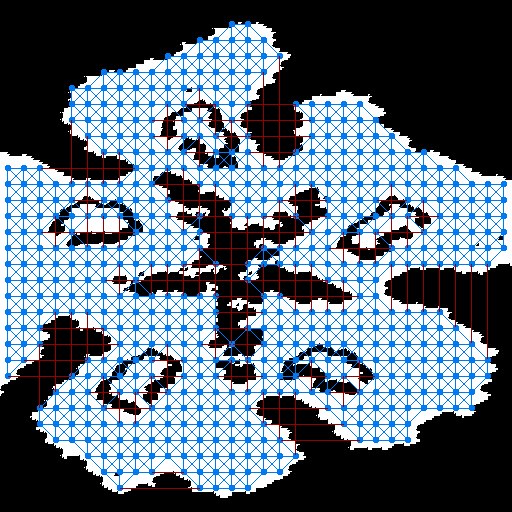
\includegraphics[width=0.22\textwidth]{img/high_path.png}
	}
	\hfill
	\subfloat{
		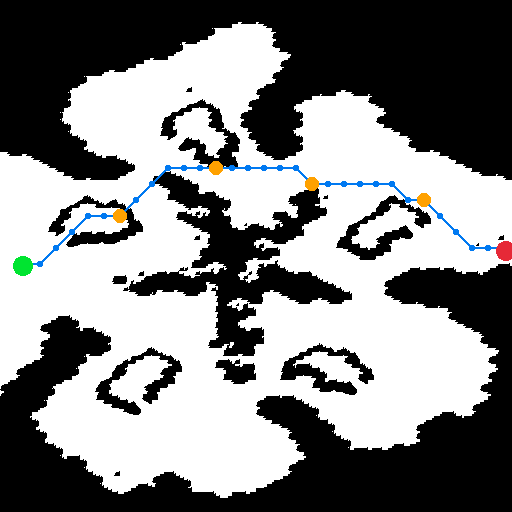
\includegraphics[width=0.22\textwidth]{img/high_graph.png}
	}
	\caption{(Left) a 32x32 mesh laid on top the \textit{StarCraft Predators} map with heavily weighted edges shown in red. (Right) The high-level path and thread starting points constructed from the left mesh, the same used for \figref{fig:ripple_example}.} 
	\label{fig:high}
\end{figure}

\mypar{Shared Lock-Free Cache}
A common technique used in many pathfinding algorithm implementations is storing some state information in the vertices themselves. 
This information typically is comprised of traversal data such as predecessor vertices, intermediate costs, etc.
For PRS specifically, each vertex can be owned by one thread and the decision was made to shift all of this runtime information into a cache structure shared between threads.
This implementation scales well, however, access to the cache needs to be synchronized to avoid data races on vertex acquisition.
To protect reads and writes, threads acquire a vertex by using an atomic \textit{compare and swap} operation to mark the vertex with its unique thread identifier and the predecessor vertex packed into a 64 bit integer. In intermediate solutions, private caches were used to try and reduce the need for synchronization. However, the additional memory initialization nullified any performance improvements in this regard. Similarly, using a single cache for both search phases requires the use of a validity tag, which needs to be checked with every access. In an attempt to remedy this, the cache was duplicated with one copy for each phase. However, this slight improvement was also offset by the increased memory initialization.
A note on implementation: special care was taken when implementing ownership of vertices in the cache. 
It took several design iterations until race conditions were no longer an issue. This especially manifested itself with setting the predecessor pointers when search threads were started too close to one another.
One more reason why load balancing of work between threads is important.

\mypar{Handling Collisions} 
A collision is detected whenever a thread fails to acquire a vertex because it's already owned by another thread.
When this happens, information about the collision, such as the threads involved, the vertex where it happened, and its predecessor, needs to be sent to a designated coordinator thread managing the overall search progress.
Search threads communicate with the coordinator via a message passing interface implemented over concurrent queues \cite{oneTBB}.
As previously mentioned, communication happens between the coordinator and search threads, but not between two search threads, thus reducing communication overhead and balancing work properly.
This implementation decision diverges from previous literature. It was observed that if a search thread handled communication, as is suggested in previous work, the \textit{refinement} phase of PRS took longer than necessary due to large differences in the size of a thread's search space.

\mypar{Vectorization}
To take advantage of vector instructions of modern x64 processors, an attempt was made to implement the core loop of fringe search using AVX512 intrisnics. 
In particular, the loading of neighboring vertices and storing the updated information in the cache was vectorized using scatter and gather operations.
Furthermore, newly-visited vertices and vertices that have their associated cost reduced by the discovery of a less expensive path, have to be inserted in the list of currently considered vertices.
The implementation of fringe search proposed by Bj\"ornsson et al. \cite{Fringe} stores the current nodes in a doubly linked list.
In this implementation, a linear array was used to take advantage of AVX512 \verb|vpcompress| instructions for appending elements efficiently without falling back to scalar code.
We measured the execution time of fringe search with a doubly-linked list and with a linear array. For the latter, both scalar and vectorized code were measured.
In measurements, using a linear array resulted in a noticeable speedup compared to the doubly linked list implementation. However, vectorized code did not provide any improvement over the scalar version.
We conjecture that this is due to the high cost of the scatter and gather operations combined with little arithmetic work.   
Therefore, in all further discussions of performance, the usage of ``vectorized'' will refer to the implementation using a linear array and not to the usage of vector instructions.
